\chapter{System Implementation and Integration}

The practical realization of the autonomous border surveillance system involves the integration of sensing, control, communication, and identification subsystems into a unified embedded platform. The implementation focuses on achieving reliable detection, accurate targeting, and real-time alert transmission. This chapter presents the hardware configuration, software architecture, and integration strategy adopted during the development of the system. It also discusses the interaction between different modules and the techniques used to ensure stable operation.

\section{Hardware Implementation}

The hardware implementation forms the physical backbone of the system. It consists of interconnected modules that perform sensing, actuation, processing, and communication.

\begin{figure}[H]
\centering
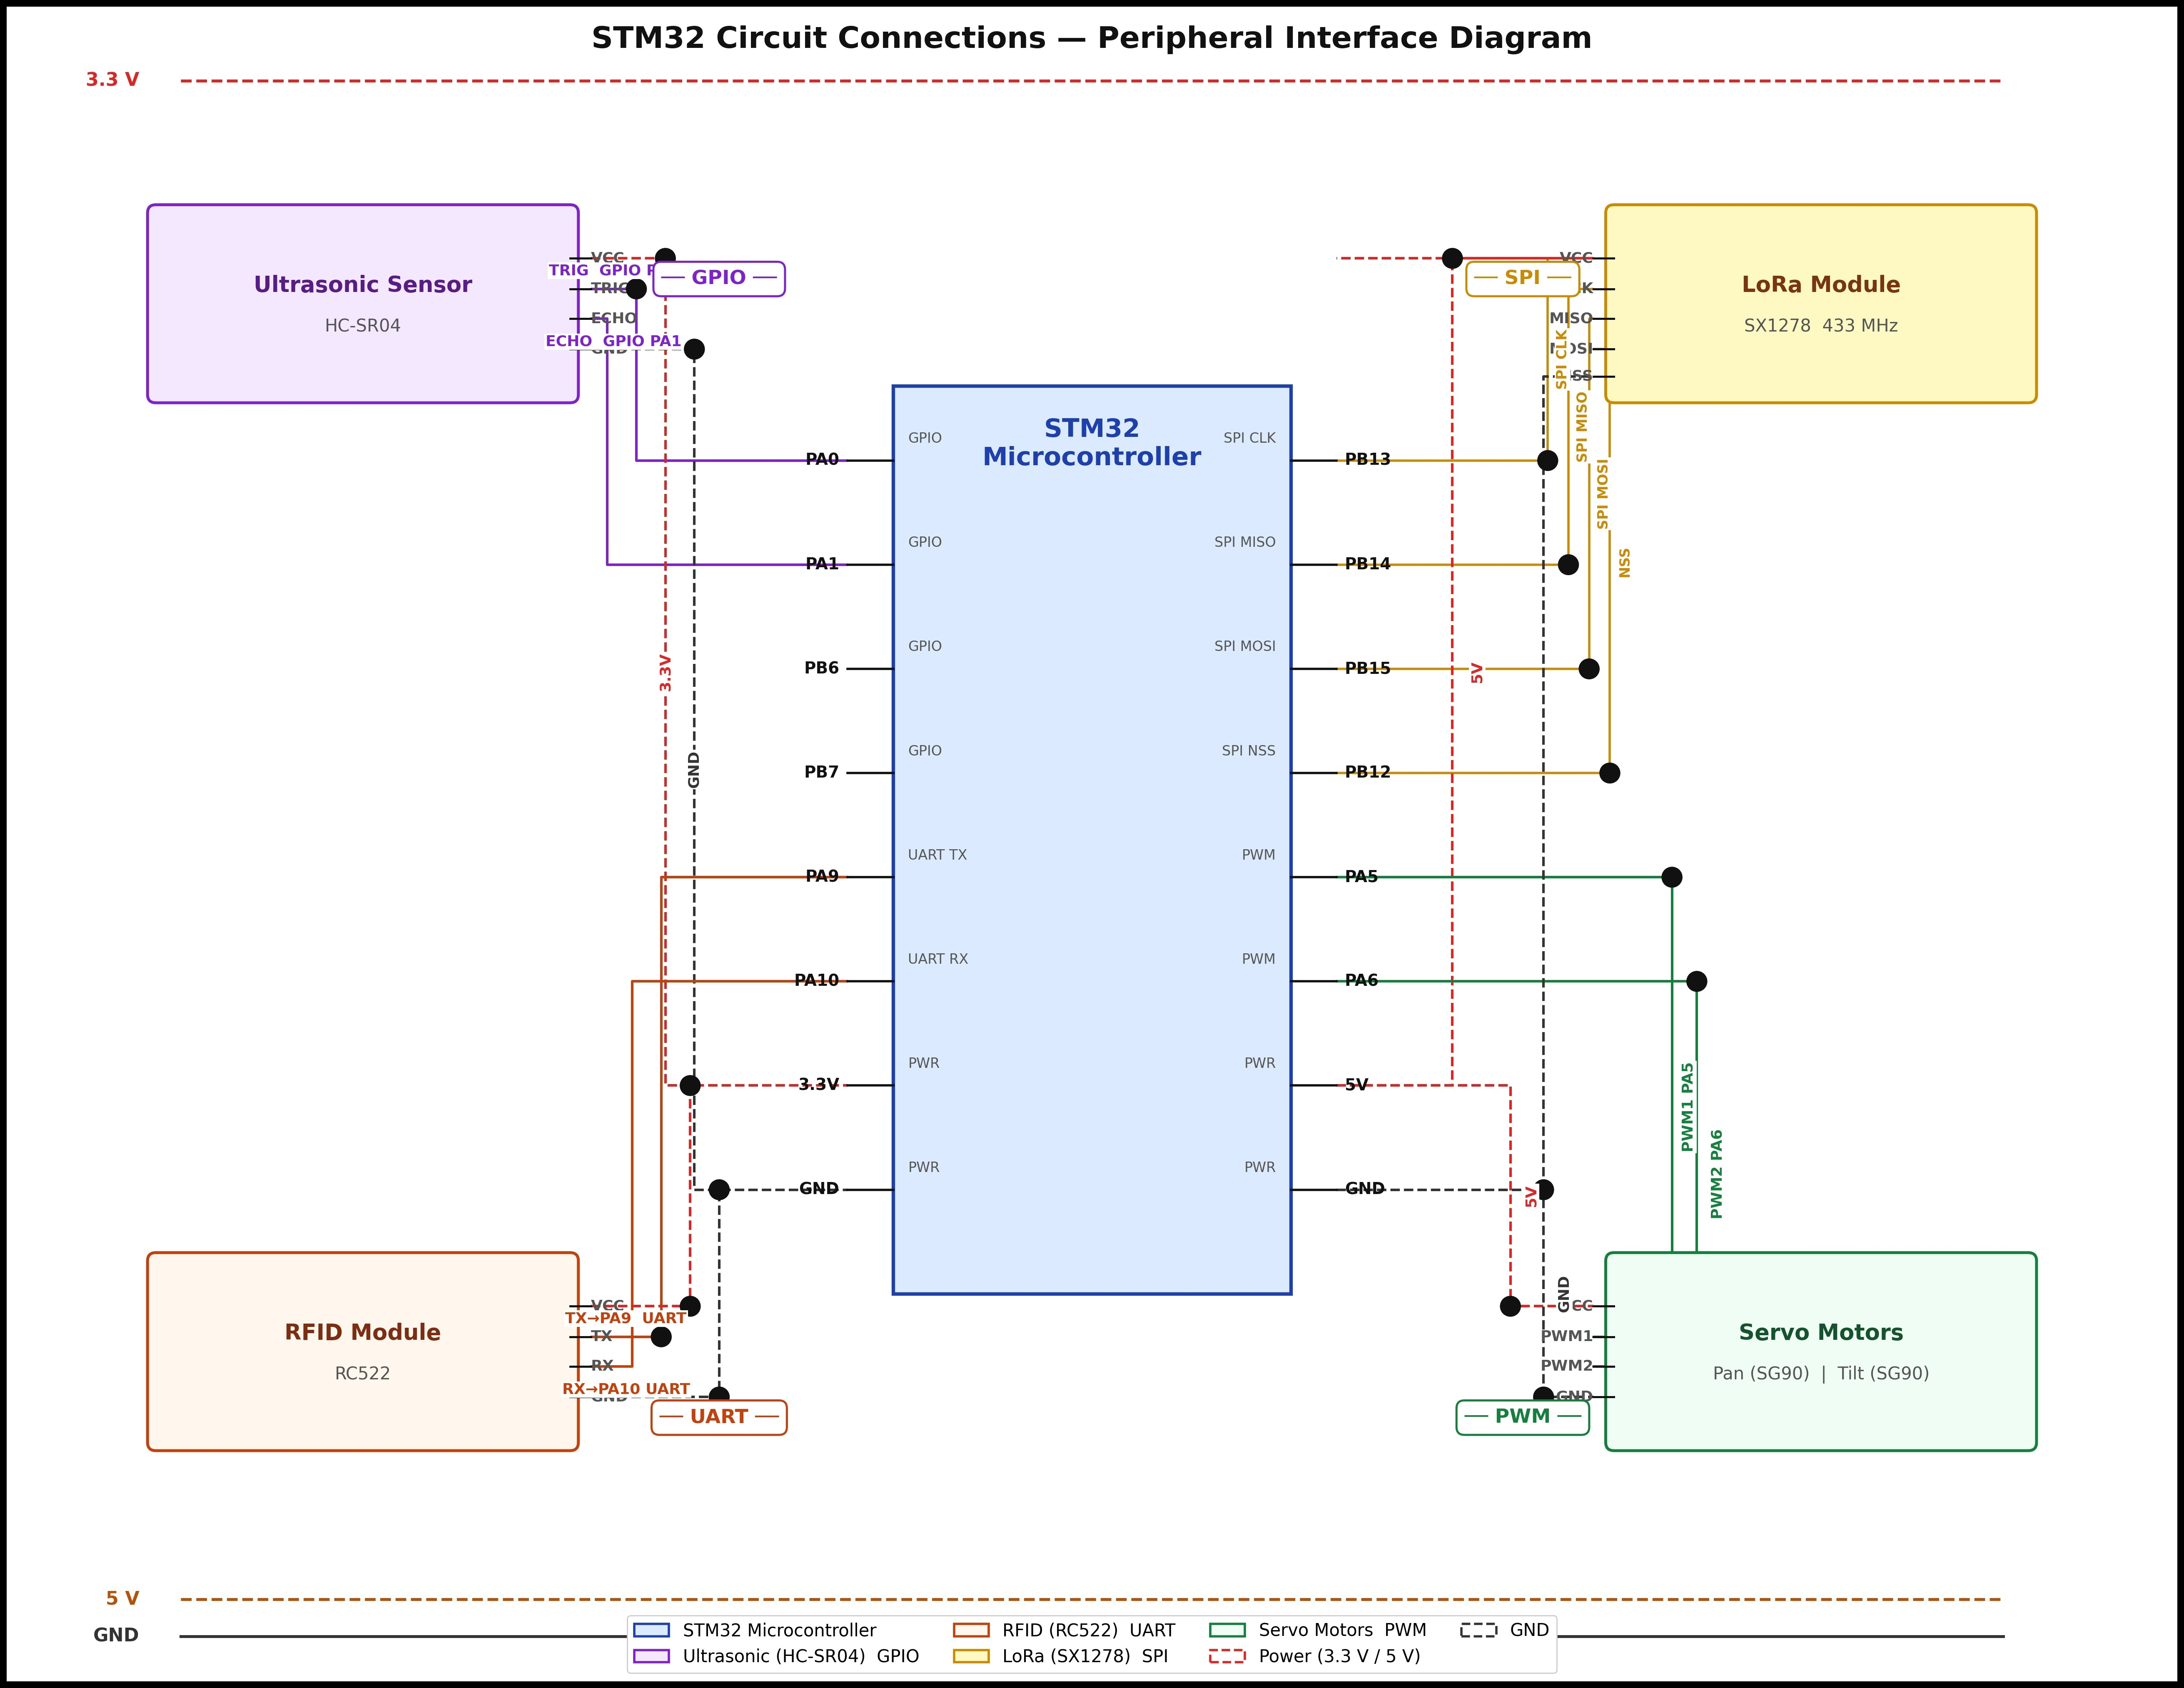
\includegraphics[width=0.75\textwidth]{figure/4.1.jpg}
\caption{Hardware implementation of the surveillance system}
\label{fig:hardware}
\end{figure}

\subsection{Microcontroller Unit}

The STM32 microcontroller serves as the central processing unit. It is responsible for:
\begin{itemize}
\item Reading sensor inputs
\item Generating PWM signals for servo control
\item Processing RFID data
\item Managing LoRa communication
\end{itemize}

The microcontroller utilizes multiple peripherals such as GPIO, timers, UART, and SPI to interface with different components.

\subsection{Ultrasonic Sensor Integration}

The HC-SR04 ultrasonic sensor is connected using two GPIO pins:
\begin{itemize}
\item Trigger pin (output)
\item Echo pin (input)
\end{itemize}

A short trigger pulse initiates the measurement, and the echo duration is captured using a timer to compute the distance.

\subsection{Servo Motor Integration}

Two servo motors are used:
\begin{itemize}
\item Pan servo for scanning
\item Tilt servo for targeting
\end{itemize}

Both servos are controlled using PWM signals generated by hardware timers. The duty cycle of the PWM signal determines the angular position of the servo.

\subsection{RFID Module Integration}

The EM-18 RFID reader is interfaced through UART communication. The module continuously transmits tag data, which is processed by the microcontroller to identify authorized users.

\subsection{LoRa Module Integration}

The SX1278 LoRa module is connected using SPI communication. Additional GPIO pins are used for control signals such as chip select and reset. The module is configured with appropriate parameters to ensure reliable long-range communication.

\subsection{Laser and Indicator System}

A laser module is used for target indication, and LEDs are used to represent system status:
\begin{itemize}
\item Green LED for authorized detection
\item Red LED for unauthorized detection
\end{itemize}

\begin{figure}[H]
\centering
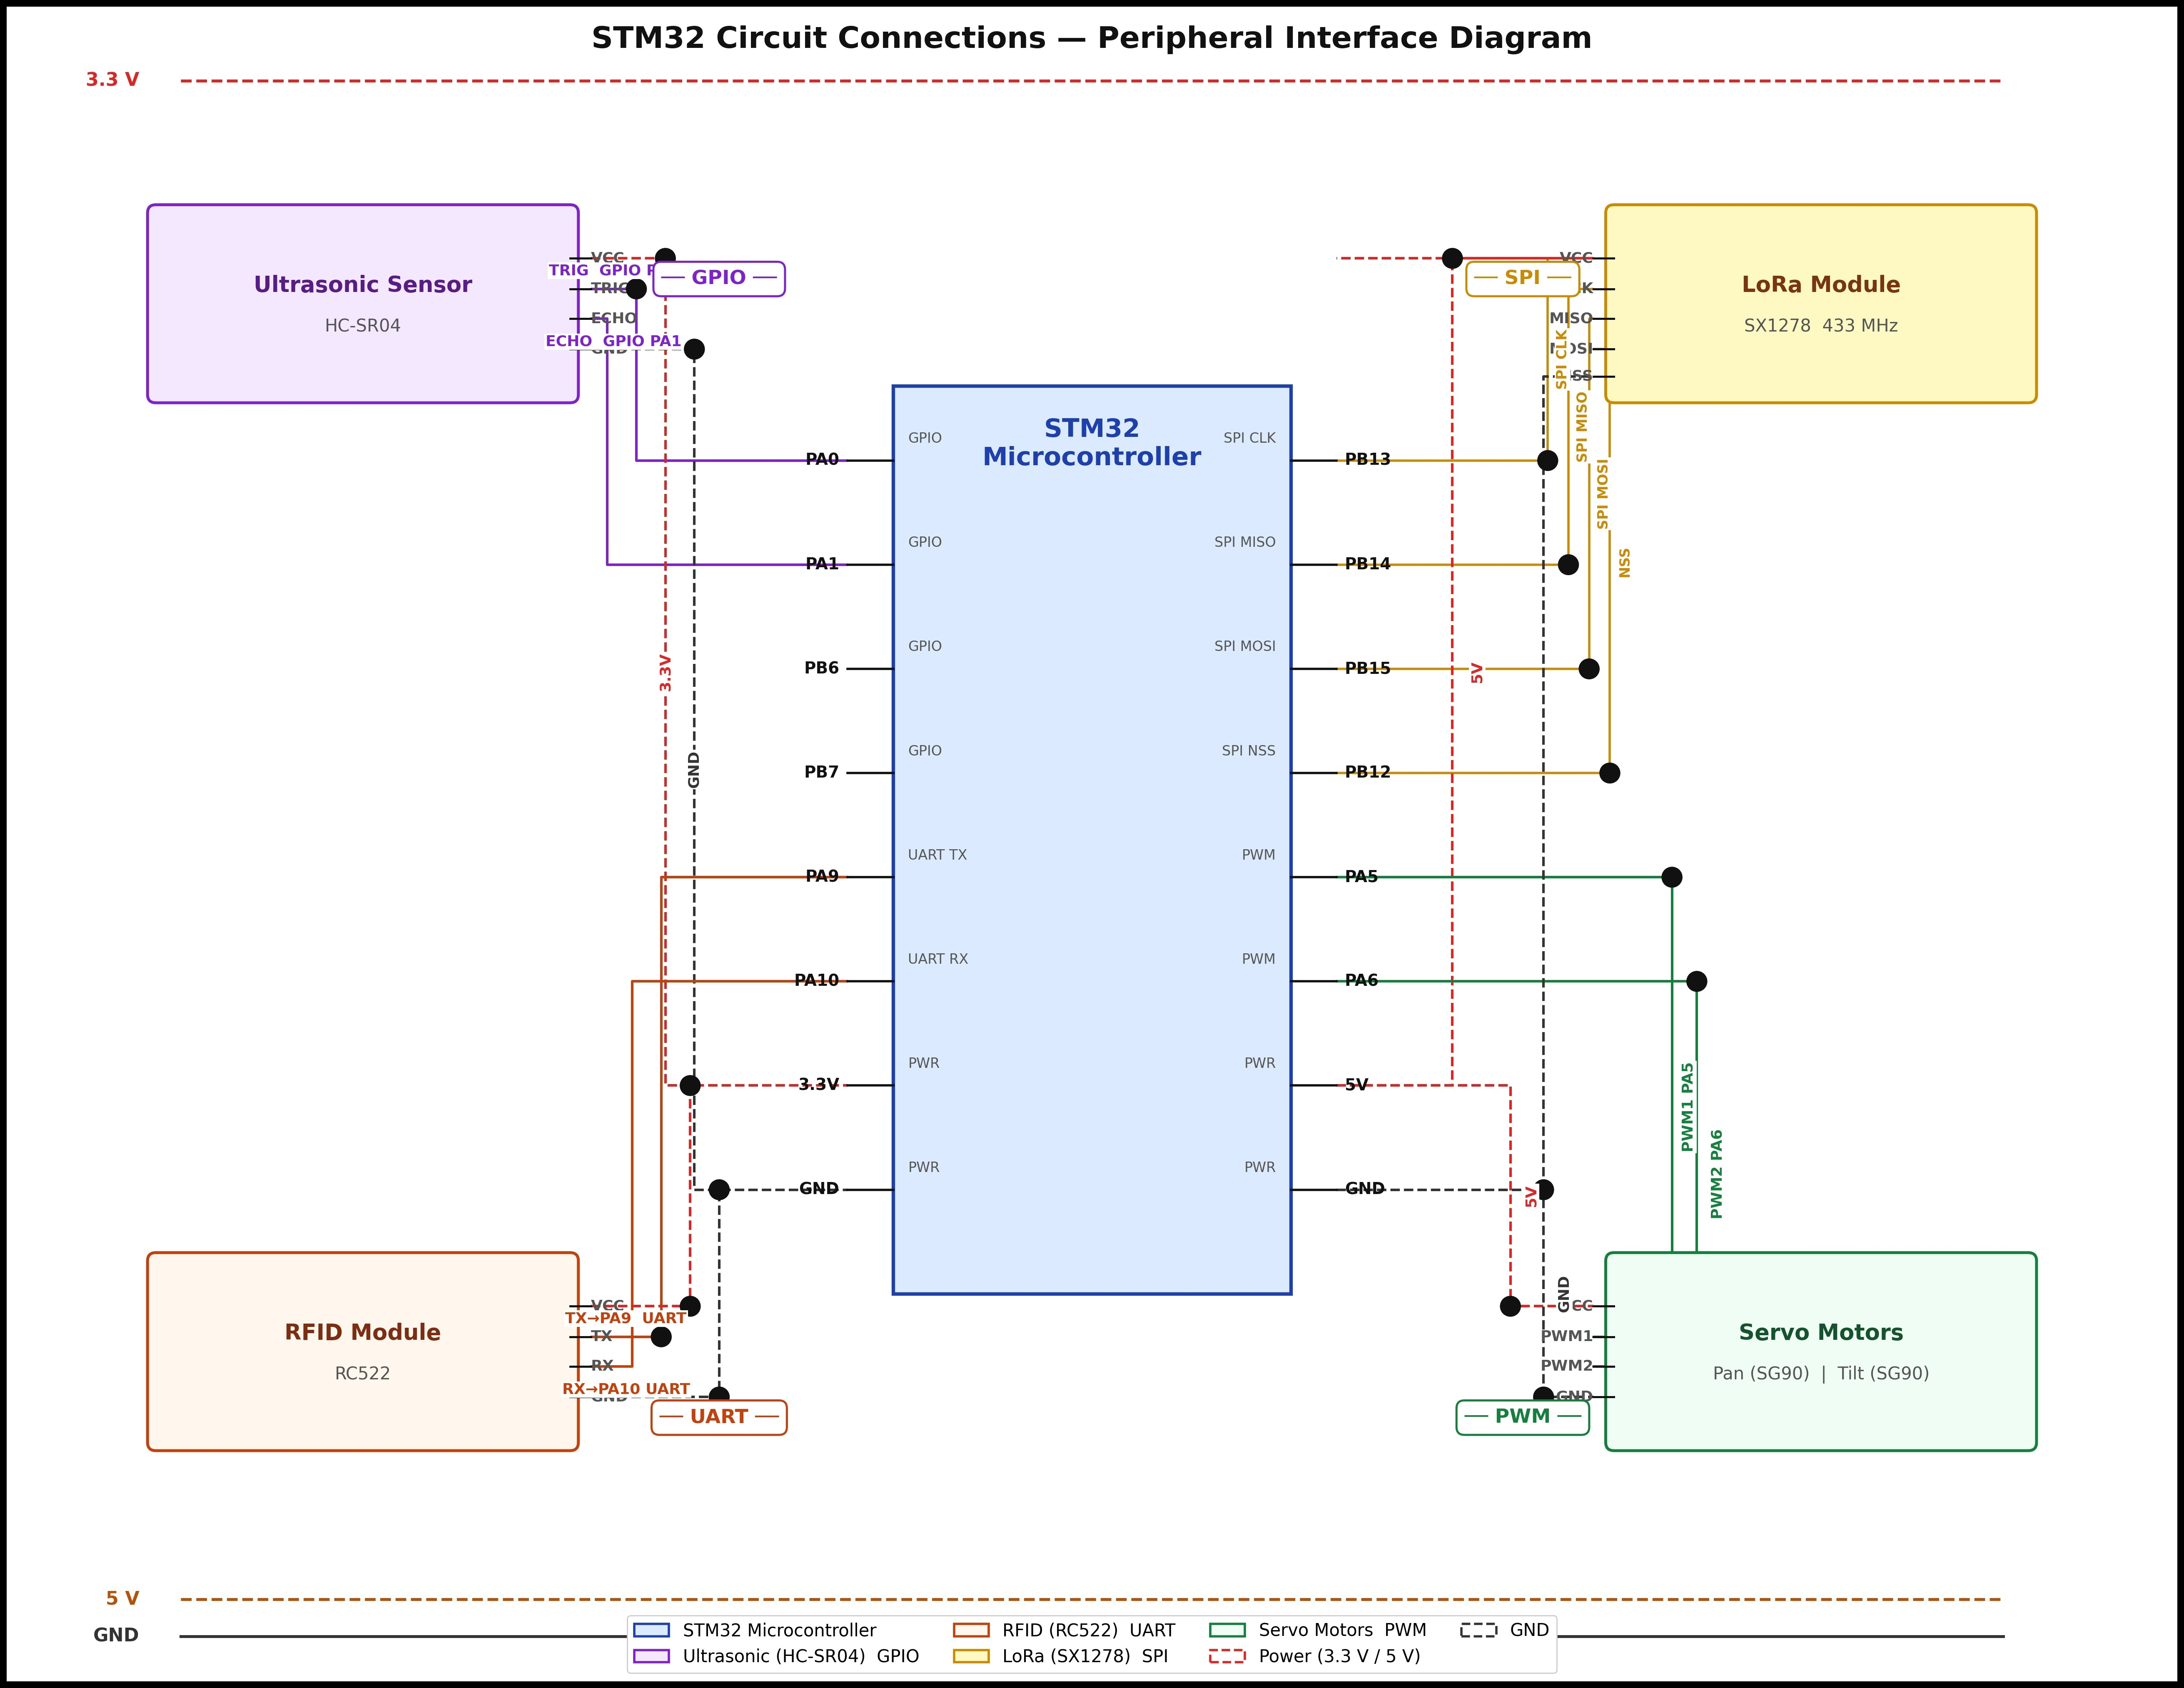
\includegraphics[width=0.75\textwidth]{figure/4.2.jpg}
\caption{Circuit diagram showing system connections}
\label{fig:circuit}
\end{figure}

\section{Software Implementation}

The software implementation is developed using embedded C and follows a modular structure.

\subsection{Initialization Phase}

During system startup, all peripherals are initialized:
\begin{itemize}
\item GPIO configuration
\item Timer setup for PWM and delay
\item UART initialization for RFID
\item SPI initialization for LoRa
\end{itemize}

This ensures that all hardware components are ready for operation.

\subsection{Main Control Loop}

The system operates continuously using a loop-based control structure. The main loop performs the following operations:

\begin{itemize}
\item Sweep servo motor across angular range
\item Measure distance using ultrasonic sensor
\item Detect target based on threshold
\item Compute targeting angle
\item Perform RFID identification
\item Trigger alert and communication
\end{itemize}

\begin{figure}[H]
\centering
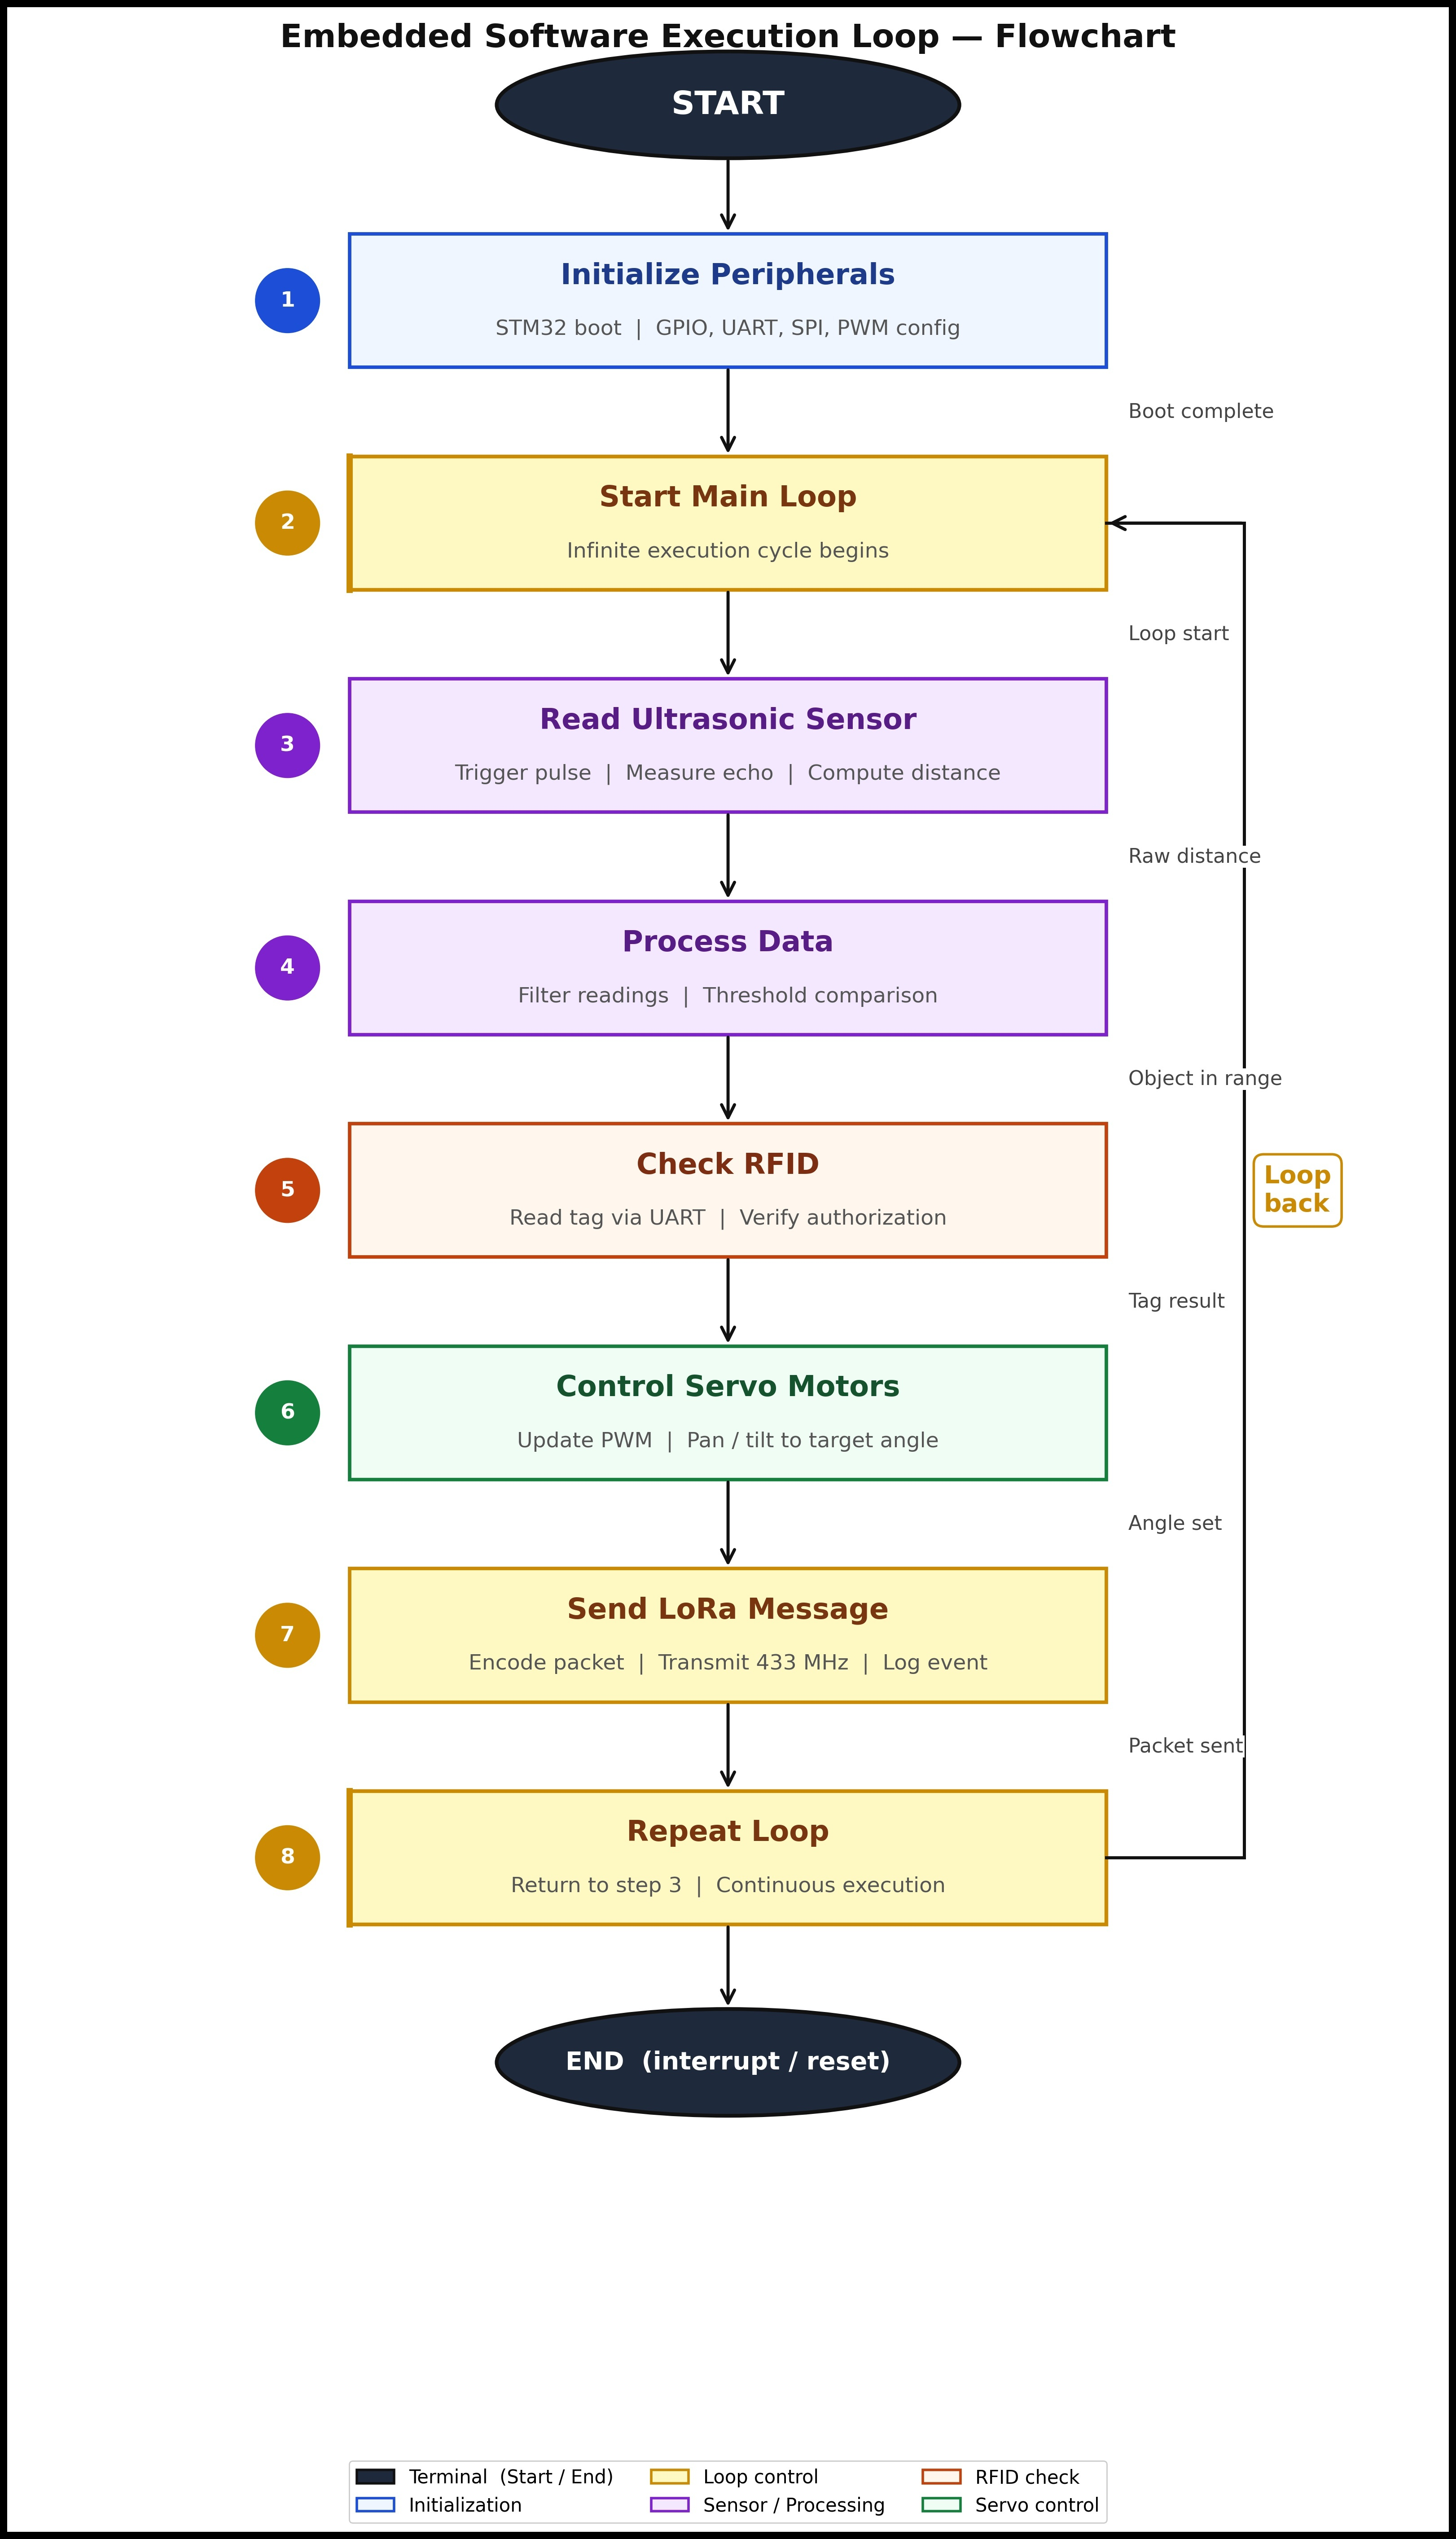
\includegraphics[width=0.7\textwidth]{figure/4.3.jpg}
\caption{Software execution flow of the embedded system}
\label{fig:software}
\end{figure}

\subsection{Distance Measurement Logic}

The ultrasonic sensor measurement involves precise timing control. A delay function is used to generate the trigger pulse, and a timer is used to measure the echo duration.

\subsection{Servo Control Logic}

Servo movement is controlled by updating PWM values. Smooth motion is achieved by gradually changing the duty cycle.

\subsection{RFID Processing Logic}

The received RFID data is stored in a buffer and compared with predefined authorized IDs. If a match is found, the system classifies the target as friendly.

\subsection{LoRa Communication Logic}

The LoRa module is initialized with predefined parameters. Messages are transmitted whenever an event occurs. The communication is designed to be reliable and energy-efficient.

\section{System Integration}

The integration of different subsystems is achieved through synchronized operation.

\begin{enumerate}
\item Sensor scans the environment
\item Object is detected within range
\item Position is calculated
\item RFID verification is performed
\item Decision is made (friendly or enemy)
\item Alert is transmitted via LoRa
\end{enumerate}

\begin{figure}[H]
\centering
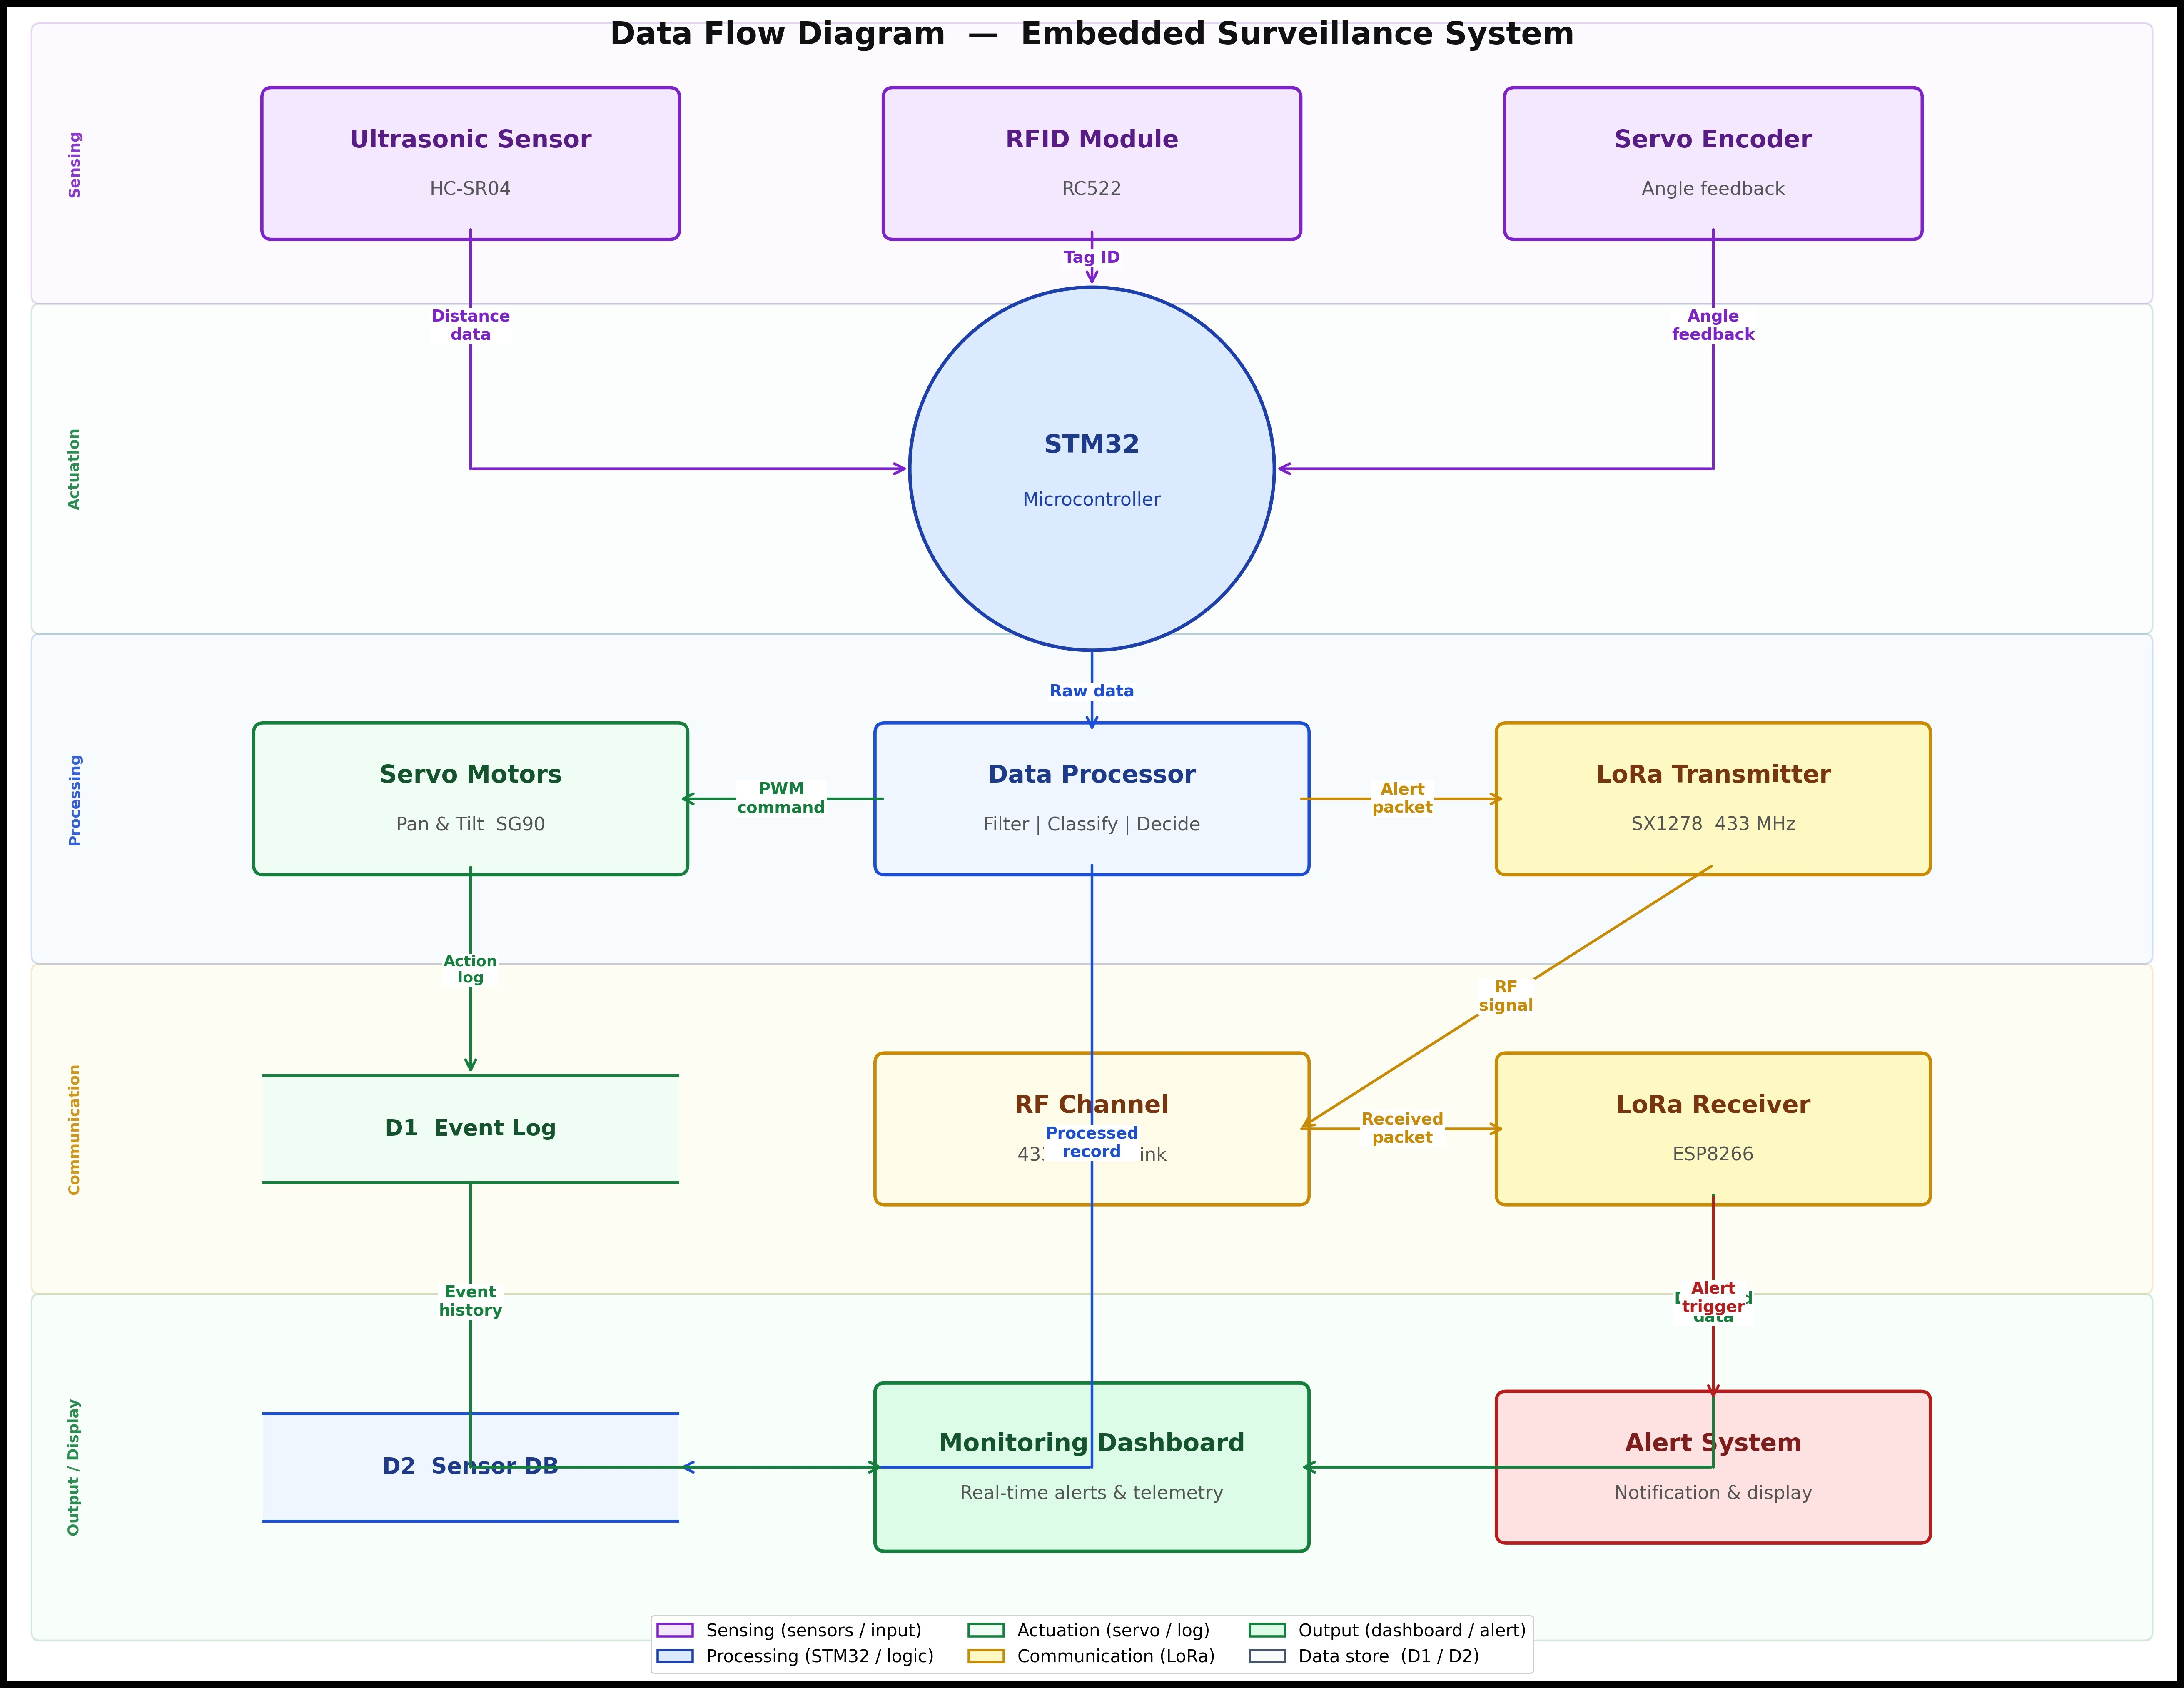
\includegraphics[width=0.75\textwidth]{figure/4.4.jpg}
\caption{Data flow representation of system components}
\label{fig:dataflow}
\end{figure}

The microcontroller coordinates all these operations to ensure seamless functioning.

\section{Top-Level Design}

The overall system can be viewed as a layered architecture:

\begin{itemize}
\item Input Layer: Sensors and RFID
\item Processing Layer: Microcontroller
\item Output Layer: Servo motors, laser, LEDs
\item Communication Layer: LoRa module
\end{itemize}

Each layer interacts with others to achieve the desired functionality.

\section{Implementation Challenges}

During implementation, several challenges were encountered:

\begin{itemize}
\item Synchronization between sensor and servo movement
\item Noise in ultrasonic readings
\item Reliable LoRa communication setup
\item Accurate RFID data processing
\end{itemize}

These challenges were addressed through calibration, filtering, and optimization techniques.

\section{Testing and Debugging}

The system was tested in stages:

\begin{itemize}
\item Individual module testing
\item Integration testing
\item Real-time testing
\end{itemize}

Debugging was performed using serial output and observation of system behavior.

\section{Chapter Summary}

This chapter presented the detailed implementation of the autonomous border surveillance system, including both hardware and software aspects. The integration of sensing, control, identification, and communication modules was discussed along with the challenges encountered during development. The next chapter presents the results, observations, and performance analysis of the implemented system.